\scanpage{221}\mspage{166}

% MS left margin beside lines 1–4
\margin{\figure{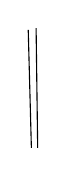
\begin{tikzpicture}[x=1mm,y=1mm]\draw (0,0)--(-0.4,15);\draw (0.8,0)--(0.6,15.2);\end{tikzpicture}}}

% MS 1–5
Mais la démonstration utilise sûrement Der 2, \deleted{\unsure{que je}} (critère d'iso par fibres, dans $\mathrm{HOT}_{\unsure{W|w}}(S)$), que je n'ai pas prouvé encore. Elle est incomplète pour le moment. Mais je peux noter dès maintenant le

% MS 6–12
\uline{Corollaire 1} (du théorème 4. p.~162) Si la flèche $S'\xrightarrow{p}S$ dans $\mathrm{Cat}$ donne lieu (pour \deleted{\unsure{$X$ fixé dans}}\inserted{tout} $f:X\longrightarrow S$ \deleted{fixé} dans $\mathrm{Cat}_{/S}$) à la formule de changement de base pour $f_!:\mathrm{HOT}_W(X)\unsure{\mathord{-}|\longrightarrow}\mathrm{HOT}_W$, alors le foncteur $p^*:X\longmapsto X\times_S S'$ de $\mathrm{Cat}_{/S}$ dans $\mathrm{Cat}_{/S'}$ \deleted{transforme} est compatible avec les localiseurs $W_S^d,W_{S'}^d$. (L'implication inverse a été vue déjà, cf. page \unsure{162|161}--163.)

% MS 13
Cela résultera du

% MS 14–16
\uline{Lemme} Soit $u:X'\longrightarrow X$ une flèche dans $\mathrm{Cat}_{/S}$. Pour que $u\in W_S^d$, il f. et s. \inserted{(si $W$ fort\textsuperscript{mt} saturé)} que pour tout $\unsure{\xi|\zeta}\in\mathrm{Hot}_W$, la flèche correspondante

% MS left of lemma
% slanted
\margin{\deleted{\unsure{le dit|le dém.}}}

% MS 17
\[
 u_{\unsure{+|*}}:p'_!(\xi_{X'})\longrightarrow p_!(\xi_X)
\]

% MS 18
soit iso. dans $\mathrm{HOT}_W(S)$.

% MS 19–21
C'est suffisant, sous réserve de saturation forte de $W$ \deleted{\unsure{$/$}}, car si $u_*$ est iso, passant aux fibres on trouve \inserted{par Dér $5'$}

% MS 22 crossed line and replacement
\[
\begin{aligned}
 &\deleted{H_{\bullet}^{\mathrm{HOT}_W}(X',\xi)\ \simeq}\\
 H_{\bullet}^{\mathrm{HOT}_W}({}_{s\backslash}X',\xi)&\longrightarrow
 H_{\unsure{\bullet|*}\deleted{\unsure{f_{\bullet}|t}}}^{\mathrm{HOT}_W}({}_{s\backslash}X,\xi),
\end{aligned}
\]

% MS 23–25
si c'est iso \deleted{\unsure{donc pour tout} $\xi$} alors $ {}_{s\backslash}X'\longrightarrow{}_{s\backslash}X$ est \inserted{par déf.} une $\mathrm{HOT}$-équivalence, ce qui signifie que c'est dans $W$ (prop.~5).

% archive sheet number: 220
